\documentclass[11pt,landscape]{article}
\usepackage{multicol}
\usepackage{calc}
\usepackage{ifthen}
\usepackage[landscape]{geometry}
\usepackage{hyperref}
\usepackage{lipsum}  

\ifthenelse{\lengthtest { \paperwidth = 11in}}
	{ \geometry{top=.5in,left=.5in,right=.5in,bottom=.5in} }
	{\ifthenelse{ \lengthtest{ \paperwidth = 297mm}}
		{\geometry{top=1cm,left=1cm,right=1cm,bottom=1cm} }
		{\geometry{top=1cm,left=1cm,right=1cm,bottom=1cm} }
	}

% Turn off header and footer
\pagestyle{empty}
 \usepackage{amsmath}

% Redefine section commands to use less space
\makeatletter
\renewcommand{\section}{\@startsection{section}{1}{0mm}%
                                {-1ex plus -.5ex minus -.2ex}%
                                {0.5ex plus .2ex}%x
                                {\normalfont\large\bfseries}}
\renewcommand{\subsection}{\@startsection{subsection}{2}{0mm}%
                                {-1explus -.5ex minus -.2ex}%
                                {0.5ex plus .2ex}%
                                {\normalfont\normalsize\bfseries}}
\renewcommand{\subsubsection}{\@startsection{subsubsection}{3}{0mm}%
                                {-1ex plus -.5ex minus -.2ex}%
                                {1ex plus .2ex}%
                                {\normalfont\small\bfseries}}
\makeatother

% Define BibTeX command
\def\BibTeX{{\rm B\kern-.05em{\sc i\kern-.025em b}\kern-.08em
    T\kern-.1667em\lower.7ex\hbox{E}\kern-.125emX}}

% Don't print section numbers
\setcounter{secnumdepth}{0}
\usepackage{circuitikz}


\setlength{\parindent}{0pt}
\setlength{\parskip}{0pt plus 0.5ex}
\usepackage{karnaugh-map}


% -----------------------------------------------------------------------

\begin{document}

\raggedright
\footnotesize
\begin{multicols*}{3}


% multicol parameters
% These lengths are set only within the two main columns
%\setlength{\columnseprule}{0.25pt}
\setlength{\premulticols}{1pt}
\setlength{\postmulticols}{1pt}
\setlength{\multicolsep}{1pt}
\setlength{\columnsep}{2pt}

\begin{center}
     \Large{\textbf{ECE253 Final Cheatsheet}}\\
     \small{\textit{Author: your mother}} \\
\end{center}



\section{Boolean Algebra}
\textbf{De Morgan's Theorem} tells us
\begin{equation}
    \overline{x\cdot y}=\overline{x}+\overline{y}, \quad\quad\quad \overline{x+y}=\overline{x}\cdot\overline{y}
\end{equation}
Inverting the inputs to an \verb!or! gate is the same as inverting the outputs to an \verb!and! gate, and the other way around. We also have: 
\begin{itemize}
    \item $(x+y)(y+z)(\overline{x}+z)=(x+y)(\overline{x}+z)$
    \item $x+yz=(x+y)(x+z)$
    \item $x+xy=x$ (Absorption)
    \item $xy+x\overline{y}=x$ (Combining)
    \item $(x+y)(x+\overline{y})=x$
    \item $ x+\overline{x}y=x+y$
    \item $x(\overline{x}+y)=xy$
    \item $xy+yz+z\overline{x}=xy+z\overline{x}$ (Consensus)
\end{itemize}

\subsection{Gates}
\begin{center}
    \begin{tabular}{c|c||c|c||c|c}
        \verb!AND! & \begin{circuitikz}[scale=0.7, transform shape] 
            \draw(0,0) node[and port] {};
        \end{circuitikz} & 

        \verb!OR! & \begin{circuitikz}[scale=0.7, transform shape] 
            \draw(0,0) node[or port] {};
        \end{circuitikz} &
        \verb!NOT! & \begin{circuitikz}[scale=0.7, transform shape] 
            \draw(0,0) node[not port] {};
        \end{circuitikz} \\ \hline
        \verb!NOR! & \begin{circuitikz}[scale=0.7, transform shape] 
            \draw(0,0) node[nor port] {};
        \end{circuitikz} &
        \verb!NAND! & \begin{circuitikz}[scale=0.7, transform shape] 
            \draw(0,0) node[nand port] {};
        \end{circuitikz} &
        \verb!XOR! & \begin{circuitikz}[scale=0.7, transform shape] 
            \draw(0,0) node[xor port] {};
        \end{circuitikz}
    \end{tabular}
\end{center}
\subsection{SOPs and POSs}
We can create boolean algebra expressions for truth tables.
\vspace{2mm}

\textbf{Minterm:} Corresponds to each row of truth table, i.e. $m_3=\overline{x_2}x_1x_0$ such that when $3=0b011$ is substituted in, $m_3=1$ and $m_3=0$ otherwise.  

\textbf{Maxterm:} They give $M_i=0$ if and only if the input is $i$. For example, $M_3=x_2+\overline{x_1}+\overline{x_0}.$

\textbf{SOP and POS:} Truth tables can be represented as a sum of minterms, or product of maxterms.
\begin{itemize}
    \item Use minterms when you have to use \verb!NAND! gates and maxterms when you have to use \verb!NOR! gates.
    \item When converting expressions to its dual, it's often helpful to negate expressions twice, or draw out the logic circuit.
\end{itemize}
\subsection{Cost}
The cost of a logic circuit is given by
\begin{equation}
    \text{cost} = \text{gates} + \text{inputs}
\end{equation}
If an inversion (\verb!NOT!) is performed on the primary inputs, then it is not included. If it is needed inside the circuit, then the \verb!NOT! gate is included in the cost.
\subsection{Karnaugh Map}
Method of finding a minimum cost expression: We can map out truth table on a grid for easier pattern recognition. Example of a four variable map is shown below:
\begin{center}
    \begin{karnaugh-map}[4][4][1][$x_2x_1$][$x_4x_3$]
        \minterms{0,1,3,4,5,7,11,14,15,10}
        \maxterms{2,6,8,9,10,12,13}
        % \indeterminants{2,5}
        \implicant{0}{5}
        \implicant{3}{11}
        \implicant{15}{10}
        % \implicant{4}{5}
    \end{karnaugh-map}
\end{center}
\vspace{-8mm}
and the representation is $\overline{x_2}\cdot\overline{x_4}+x_2 \cdot x_1+\overline{x_4} \cdot x_2$ when using \textit{minterms}. To use \textit{maxterms}, we take the intersection of sets that don't include blocks of $0$s. For example, $(\overline{x_2}\cdot \overline{x_1})(\overline{x_2}+x_1+x_4).$ Some \textit{rules}: 
\begin{itemize}
    \item Side lengths should be powers of $2$ and be as large as possible.
    \item Use \textbf{graycoding}: adjacent rows/columns should share one bit.
\end{itemize}
\subsubsection{Minimization Procedure}
\begin{enumerate}
    \item Generate all prime implicants for given function $f$
    \item Find the set of essential prime implicants
    \item Determine the nonessential prime implicants that should be added.
\end{enumerate}
\subsection{Common Logic Gates}
\begin{itemize}
    \item \textbf{Mux 2$\rightarrow$1:} $\verb#mux2to1#(s,x_0,x_1) = \overline{s}x_0+sx_1$
    \item \textbf{Not:} \verb#not(x)=nand(x,x)=nor(x,x)#
    \item \verb!XOR! acts as modular arithmetic.
    \item Multiplexers are functionally complete. $\verb!AND!=mux(x,y,1)$, $\verb!OR!=mux(x,0,y).$
\end{itemize}
\subsection{RS Latch}
Sequential circuits depend on sequence of inputs. A \textbf{SR Latch} are cross-coupled \verb!NOR! gates.
\vspace{2mm}
% \begin{center}
    {
    \begin{multicols}{2}
        \begin{center}
            \begin{circuitikz} \draw
                (0,2) node[nor port] (NOR1) {}
                (1,2) node[anchor=east] {Q}
                (1,0) node[anchor=east] {$\overline{Q}$}
                (0,0) node[nor port] (NOR2) {}
                (NOR1.in 1) node[anchor=east] {R}
                (NOR2.in 2) node[anchor=east] {S}
                (NOR1.out) -- ++(0,-0.5) -- ($(NOR2.in 1) +(0,0.5)$) -- (NOR2.in 1)
                (NOR2.out) -- ++(0,+0.5) -- ($(NOR1.in 2) +(0,-0.5)$)--(NOR1.in 2)
                ;\end{circuitikz}
        \end{center}


        \begin{center}
            \begin{tabular}{c|c|c|c}
                S & R & Q & $\overline{Q}$ \\ \hline
                0 & 0 & 0/1 & 1/0 \\
                0 & 1 & 0 & 1 \\ 
                1 & 0 & 1 & 0 \\ 
                1 & 1 & 0 & 0
           \end{tabular}
        \end{center}
        \vspace{-2mm}
        \scriptsize When $S=R=0$, it stores the last $Q$ value. In practice, we should not have $S=R=1$.
    \end{multicols}
}
\subsection{Gated D Latch and Clock Signal}
{
    \begin{multicols}{2}
        \begin{center}
            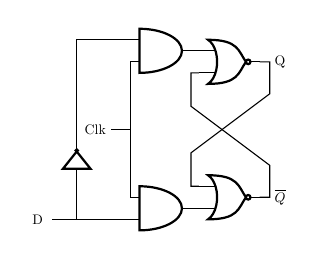
\begin{tikzpicture}[scale=0.5, transform shape]
 
                % Draw and gates
                \node[and port] (and1) at (0,2) {};
                \node[and port] (and2) at (0,-2) {};
                 
                % Draw nor gates
                \draw (and1.out) -- ++(0.2,0) node
                [
                    nor port,
                    anchor=in 1
                ] (nor1) {};
                 
                \draw (and2.out) -- ++(0.2,0) node
                [
                    nor port,
                    anchor=in 2
                ] (nor2) {};
                 
                \draw (nor1.in 2) -| ++ (-0.2,-0.85) -- ++(2,-1.5) coordinate(a) |- (nor2.out);
                \draw (nor2.in 1) -| ++ (-0.2,0.85) -- ++(2,1.5) |- (nor1.out);
                 
                % Clock
                \draw (and1.in 2) -- (and2.in 1)node[midway](clk){};
                \draw (clk.center) -- ++(-0.5,0) node[left]{Clk};
                 
                % Output labels
                \draw (nor1.out -| a) node[right]{Q};
                \draw (nor2.out -| a) node[right]{$\overline{Q}$};
                 
                \draw (and2.in 2) -- ++(-2,0) coordinate(a2) node[left=0.1cm]{D};
                 
                % Not port
                \node
                [
                    not port,
                    rotate=90,
                    scale=0.5,
                ](not) at (-2.75,-0.75){};
                 
                \draw (not.in) |- (a2) (not.out) |- (and1.in 1)  ;
                 
                \end{tikzpicture}
        \end{center}


        \begin{center}
            \begin{tabular}{c|c}
                Clk & $Q(t+1)$ \\ \hline
                0 & Q(t) \\
                1 & D
           \end{tabular}
        \end{center}
        \vspace{-3mm}
    \end{multicols}
}

% \end{center}
\subsection{D Flip Flops}
Consists of two gated D latches, connected in series and both connected to the same clock. However, clock input for the first D latch is inverted. When the clock rises up, $Q$ stores value of $D$.
\subsection{T Flip Flops}
\begin{multicols}{2}
    \includegraphics[width=1.1\linewidth]{figures/T.png}
    \begin{center}
        \begin{tabular}{c|c|c}
        clk & $Q(t+1)$ \\ \hline
        $\uparrow$ & \verb!T^Q(t)! 
   \end{tabular}
    \end{center}
\end{multicols}
\subsection{SystemVerilog}
\subsubsection{Logic Operators}
\begin{center}
    \begin{tabular}{c|c||c|c}
        \verb!bitwise AND! & \verb!&! &
        \verb!bitwise OR! & \verb!|! \\ \hline
        \verb!bitwise NAND! & \verb!~&! &
        \verb!bitwise NOR! & \verb!~!!  \\ \hline
        \verb!bitwise XOR! & \verb!^! &
        \verb!bitwise XNOR! & \verb!~^! \\ \hline
        \verb!logical negation! & \verb!!! &
        \verb!bitwise negation! & \verb!~! \\ \hline 
        \verb!concatenation! & \verb!{}! &
        \verb!replication! & \verb!{{}}! 
    \end{tabular}
\end{center}
\begin{itemize}
    \item \verb!reduction! operators are put at the start and output a scalar.
    \item \verb!bitwise! operators 
    \item \verb!blocking assignment =!: executed in the order they are specified.
    \item\verb!Nonblock assignments <=! executed in parallel.
    \item Use \verb!logic! instead of \verb!reg/wire! (4-state type)
    \item Use \verb!always_comb! for combinational, \verb!always_ff! for sequential logic
\end{itemize}
\newpage 
\subsubsection{Case Statements}
\begin{verbatim}
module mux(
    input logic [2:0] MuxSelect,
    input logic [4:0] Input,
    output logic Out
);
    always_comb begin
        case (MuxSelect)
            3'b000: Out = Input[0];
            // ...
            3'b100: Out = Input[4];
            default: Out = 1'bx;
        endcase
    end
endmodule
\end{verbatim}
\subsubsection{Half Adder}
\begin{verbatim}
module HA(
    input logic x, y,
    output logic s, c
);
    assign s = x ^ y;
    assign c = x & y;
endmodule
\end{verbatim}
\subsubsection{Full Adder}
\begin{verbatim}
module FA(
    input logic a, b, c_in,
    output logic s_out, c_out
);
    logic w1, w2, w3;
    HA u0(.x(a), .y(b), .s(w1), .c(w2));
    HA u1(.x(c_in), .y(w1), .s(s_out), .c(w3));
    assign c_out = w2 | w3;
endmodule
\end{verbatim}
\subsection{D Flip Flop}
\begin{verbatim}
module D_ff(
    input logic D, clk,
    output logic Q
);
    always_ff @(posedge clk)
        Q <= D;
endmodule
\end{verbatim}
\subsection{T Flip Flops}
\begin{verbatim}
module t_ff(
    input logic Clock, Clear_b, T,
    output logic Q
);
    always_ff @(posedge Clock, negedge Clear_b) begin
        if (Clear_b == 1'b0)
            Q <= 1'b0;
        else
            Q <= T ^ Q;
    end
endmodule
\end{verbatim}
\subsection{Registers}
\begin{verbatim}
module reg8(
    input logic clk,
    input logic [7:0] D,
    output logic [7:0] Q
);
    always_ff @(posedge clk)
        Q <= D;
endmodule
\end{verbatim}
\subsection{ModelSim Do Files}
\begin{verbatim}
# set working dir, where compiled verilog goes
vlib work
# compile all verilog modules in mux.v to working
# dir could also have multiple verilog files
vlog mux.v
#load simulation using mux as the
# top level simulation module
vsim mux
#log signals and add signals to waveform window
log {/*}
# add wave {/*} would add all items in
# top level simulation module
add wave {/*}
# set input values using the force command
# signal names need to be in {} brackets
force {SW[0]} 0
force {SW[1]} 0
run 10ns
\end{verbatim}
\textbf{ModelSim and Other Lab Things}
\begin{itemize}
    \item FGPA: Field Programmable Gate Array
    \item To repeat signals, use this syntax: 
    \begin{verbatim}
force {MuxSelect[2]} 0 0ns, 1 {4ns} -r 8ns
    \end{verbatim}
    \vspace{-4mm}
    which starts at $0$ at 0ns, $1$ at 4ns, and repeats every $8$ ns.
    \item On the \verb!DE1-SoC! board, hex thing is red if $0$ and white if $1$.
\end{itemize}
\subsection{Frequency Dividers}
\begin{itemize}
    \item To half the frequency, connect $\overline{Q}$ to $D$ on the same gated D latch.
    \item To quarter the frequency, connect $\overline{Q}$ to the clock of the next gated D latch (which is set up the same as the half frequency case).
    \item To reduce frequency by $2k$, connect $k$ D latches connected in series ($D$ to $Q$) and to the same clock. First $D$ is connected to last $\bar{Q}$. The last $Q$ will have a reduced frequency of $2k$.
\end{itemize}
\subsection{Resets}
\begin{itemize}
    \item Active High/Low: Resets when Signal is 1/0
    \item Synchronous High/Low: Resets during positive/negative edge
\end{itemize}
\section{Finite State Machines}
\subsection{Steps}
\begin{multicols}{2}
    \begin{enumerate}
        \item State Diagram
        \item State Table
        \item State Assignment
        \item State-Assigned Table
        \item Synthesize Circuit
        \item Celebrate!
    \end{enumerate}
\end{multicols}
\subsection{Step 1: State Diagram Example}
\begin{center}
    \includegraphics[width=0.6\linewidth]{figures/fsm.png}
\end{center}
\subsection{Step 2: State Table Example}
\begin{center}
    \begin{tabular}{c|cc|c}
        Present State & \multicolumn{2}{c|}{Next State} & Output ($z$) \\ 
        A & A & B& 0 \\ 
        B & A & C & 0 \\ 
        $\vdots$ & $\vdots$ & $\vdots$ & $\vdots$ \\
        G & A & C & 1
    \end{tabular}
\end{center}
\subsection{Step 3: State Assignment Example}
\begin{itemize}
    \item Using \textbf{one-hot encoding:} Choose number of flip flops: $7$ (since 7 states)
    \item Choose state codes:
    \begin{itemize}
        \item A = 0000001, B=0000010, $\dots$, G=1000000
    \end{itemize}
\end{itemize}
Alternatively use 3 flip flops to represent state codes as 000, 001, 010, etc.

\newpage 

\subsection{Step 4: State-Assigned Table Example}
By convention, use $y$ for input and $Y$ for output.
\begin{tabular}{c|cc|c}
    $y_3y_2y_1$ & $Y_3Y_2Y_1$ $(W=0)$ & $Y_3Y_2Y_1$ $(W=1)$ & z \\ 
    000 & 000 & 001 & 0 \\ 
    001 & 000 & 010 & 0 \\
    $\vdots$ & $\vdots$ & $\vdots$ & $\vdots$ \\
    110 & 000 & 010 & 1
\end{tabular}
\subsection{Step 5: Synthesize Example}
We first write boolean algebra expressions for the outputs $Y_n=f_n(y_1,y_2,y_3,W$) and $z=g(y_1,y_2,y_3)$. For each flip flop $i$, the input is $Y_i$ and the output is $y_i$. The output then branches off into two paths:
\begin{itemize}
    \item The first path goes into the function $g(y_1,y_2,y_3)$ and leads to output $z$
    \item The second path goes into the function $f_nm(y_1,y_2,y_3,W)$ and \textbf{loops back} to $Y_n.$
\end{itemize}
The D flip flops are connected to same clock and reset signal.
\subsection{Execution in SystemVerilog}
\begin{verbatim}
module FSM(
    input logic Clock, Resetn, w,
    output logic z,
    output logic [3:0] CurState
);

logic [3:0] y_Q, Y_D;

typedef enum logic [3:0] {
    A = 4'b0000,
    B = 4'b0001,
    // ...
    G = 4'b0110
} state_t;

always_comb begin
    case (y_Q)
        A: Y_D = w ? B : A;
        // ...
        G: Y_D = w ? C : A;
        default: Y_D = A;
    endcase
end

always_ff @(posedge Clock) begin
    if (!Resetn)
        y_Q <= A;
    else
        y_Q <= Y_D;
end

assign z = (y_Q == F) | (y_Q == G);
assign CurState = y_Q;

endmodule
\end{verbatim}
\section{RISC-V Assembly}
\subsection{Registers}
\vspace{-2mm}
{\footnotesize
\begin{itemize}\setlength\itemsep{-0.5em}
    \item x0 (zero): Hardwired zero, x1 (ra): Return address, x2 (sp): Stack pointer
    \item x5-x7, x28-x31 (t0-t6): Temporary (caller-saved)
    \item x8-x9, x18-x27 (s0-s11): Saved (callee-saved)
    \item x10-x17 (a0-a7): Function args/return values
    \item x3 (gp): Global pointer, x4 (tp): Thread pointer
\end{itemize}}
\subsection{Instructions}
Let \verb!a0=1!, \verb!a1=2!, \verb!a2=0b1010!.
\begin{center}
    \begin{tabular}{c|c|c}
    Instruction & Example & Result \\ 
    \verb!ADDI! & \verb!addi a3, zero, 3! & \verb!a3 = 3     !\\ 
    \verb!ADD! & \verb!add a3, a0, a0! & \verb!a3 = 1 + 1 !\\
    \verb!SUB! & \verb!sub a3, a0, a0! & \verb!a3 = 1 - 1 !\\
    \verb!MUL! & \verb!mul a3, a0, a0! & \verb!a3 = 1 * 1 !\\
    \verb!SLLI! & \verb!slli a3, a2, 1! & \verb!a3 = 0b10100! \\ 
    \verb!SRLI! & \verb!srli a3, a2, 1! & \verb!a3 = 0b0101! \\
    \verb!SRAI! & \verb!srai a3, a2, 1! & \verb!a3 = 0b1101! \\
    \verb!AND! & \verb!and a3, a1, a0! & \verb!a3 = (1 and 2) = 0! \\
    \end{tabular}
\end{center}
\subsection{Memory Stuff}
\vspace{-2mm}
{\footnotesize
\begin{itemize}\setlength\itemsep{-0.5em}
    \item \verb!JAL!: Jump and Link - stores return address in \verb!ra! (x1)
    \item \verb!JALR!: Jump and Link Register - indirect jump
    \item Stacks: Manual push/pop: \verb!addi sp, sp, -8! then \verb!sw a0, 0(sp)!
    \item Each instruction is 4 bytes (32-bit) in RV32.
\end{itemize}}
\subsection{Load and Store}
\vspace{-2mm}
{\footnotesize
\begin{itemize}\setlength\itemsep{-0.5em}
    \item \verb!lw a0, offset(a1)!: Load word; \verb!sw a0, offset(a1)!: Store word
    \item \verb!la a0, label!: Load address (pseudo-instruction)
    \item \verb!lb/lbu! - load byte (signed/unsigned), \verb!lh/lhu! - load halfword
    \item \verb!sb! - store byte, \verb!sh! - store halfword
\end{itemize}}
\subsection{Conditionals}
\vspace{-2mm}
{\scriptsize
RISC-V has no flags. Branch instructions: \verb!beq! (equal), \verb!bne! (not equal), \verb!blt/bge! (less/greater signed), \verb!bltu/bgeu! (unsigned). Set: \verb!slt!, \verb!slti!, \verb!sltu!, \verb!sltiu!.
}
\subsection{Interrupts}
\vspace{-2mm}
{\footnotesize
\begin{enumerate}\setlength\itemsep{-0.5em}
    \item Set \verb!mtvec! CSR (trap vector)
    \item Enable interrupts in \verb!mstatus! (MIE bit)
    \item Enable sources in \verb!mie! CSR
    \item Configure PLIC/CLIC
    \item Save context on trap entry
    \item Read \verb!mcause! CSR for cause
    \item Handle in ISR, clear PLIC pending bit
    \item Restore context, return with \verb!mret!
\end{enumerate}}
\section{RISC-V Assembly Example Code}
\subsection{Enabling Interrupts}
\vspace{-2mm}
{\scriptsize
\begin{verbatim}
li sp, 0x10000        # Initialize stack
la t0, trap_handler
csrw mtvec, t0        # Set trap vector
li t0, 0x8
csrs mstatus, t0      # Enable interrupts (MIE)
li t0, 0x800
csrs mie, t0          # Enable external int (MEIE)
li t0, 0xFF20058
li t1, 0b1001
sw t1, 0(t0)          # Enable key3, key0
\end{verbatim}}
\subsection{Check Cause of Interrupt}
\vspace{-2mm}
{\scriptsize
\begin{verbatim}
trap_handler:
    addi sp, sp, -32
    sw t0, 0(sp); sw t1, 4(sp); sw a0, 8(sp)
    sw a1, 12(sp); sw ra, 16(sp)
    csrr t0, mcause       # Read cause
    li t1, 0x8000000B
    bne t0, t1, error_trap
    jal ra, key_isr
    j exit_trap
error_trap:
    j error_trap
exit_trap:
    lw t0, 0(sp); lw t1, 4(sp); lw a0, 8(sp)
    lw a1, 12(sp); lw ra, 16(sp)
    addi sp, sp, 32
    mret
\end{verbatim}}
\subsection{ISR Subroutine}
\vspace{-2mm}
{\scriptsize
\begin{verbatim}
key_isr:
    addi sp, sp, -20
    sw t2, 0(sp); sw t3, 4(sp)
    sw t4, 8(sp); sw t5, 12(sp)
    la t5, CURR_VALUE
    lw t4, 0(t5)
    li t2, 0xFC20005C
    lw t3, 0(t2)
    li t0, 0b1000
    bne t3, t0, key0
    beq t4, zero, endisr
    addi t4, t4, -1
    sw t4, 0(t5)
    j endisr
key0:
    # code for key 0
endisr:
    lw t2, 0(sp); lw t3, 4(sp)
    lw t4, 8(sp); lw t5, 12(sp)
    addi sp, sp, 20
    ret
\end{verbatim}}
\subsection{Polled IO with Timer}
\vspace{-2mm}
{\scriptsize
\begin{verbatim}
.text
.globl _start
_start:
    li a0, 0xFFFEC600
    li a1, 200000000
    sw a1, 0(a0)
    li a1, 0b111
    sw a1, 8(a0)
    li s0, 0; li s1, 0; li s2, 0  # sec,min,hr
poll:
    lw a1, 12(a0)
    beq a1, zero, poll
    sw a1, 12(a0)
    addi s0, s0, 1
    li t0, 60
    bne s0, t0, poll
    li s0, 0
    addi s1, s1, 1
    bne s1, t0, poll
    li s1, 0
    addi s2, s2, 1
    li t0, 24
    bne s2, t0, poll
    li s2, 0
    j poll
\end{verbatim}}
\subsection{Exception Vector Table}
\vspace{-2mm}
{\scriptsize
\begin{verbatim}
.align 2
trap_vector:
    j trap_handler  # Direct: all to one handler
# Vectored: mtvec.MODE=1, base + 4*cause
# 0x00:Exception 0x04:Supervisor SW int
# 0x0C:Machine SW int 0x14:Supervisor timer
\end{verbatim}}
\subsection{Find Sum with Recursion}
\vspace{-2mm}
\begin{multicols}{2}
{\scriptsize
\begin{verbatim}
.globl _start
_start:
    li sp, 0x20000
    la s0, N
    lw a0, 0(s0)
    li a1, 0
    jal ra, findsum
    add a1, a1, a0
end: j end
findsum:
    addi sp, sp, -8
    sw a0, 0(sp); sw ra, 4(sp)
    li t0, 2
    blt a0, t0, return
    addi a0, a0, -1
    jal ra, findsum
    add a1, a1, a0
return:
    lw a0, 0(sp); lw ra, 4(sp)
    addi sp, sp, 8
    ret
.data
N: .word 5
\end{verbatim}}
\end{multicols}
\subsection{Fibonacci with Recursion}
\vspace{-2mm}
\begin{multicols}{2}
{\scriptsize
\begin{verbatim}
.data
N: .word 10
.text
.globl _start
_start:
    li sp, 0x20000
    la s0, N; lw a0, 0(s0)
    li a1, 0; li a2, 0
    jal ra, fib
end: j end
fib:
    addi sp, sp, -12
    sw a0, 0(sp); sw a2, 4(sp)
    sw ra, 8(sp)
    li t0, 2
    bge a0, t0, recur
    mv a1, a0
    lw a0, 0(sp); lw a2, 4(sp)
    lw ra, 8(sp)
    addi sp, sp, 12
    ret
recur:
    addi a0, a0, -1
    jal ra, fib
    mv a2, a1
    addi a0, a0, -1
    jal ra, fib
    add a1, a1, a2
    lw a0, 0(sp); lw a2, 4(sp)
    lw ra, 8(sp)
    addi sp, sp, 12
    ret
\end{verbatim}}
\end{multicols}
\end{multicols*}
\end{document}
